\documentclass[12px]{article}
\usepackage{graphicx} % Required for inserting images

\usepackage[T2A]{fontenc}
\usepackage[utf8]{inputenc}
\usepackage[english, russian]{babel}
\usepackage{amsmath}

\usepackage{geometry}
 \geometry{
 a4paper,
 total={170mm,257mm},
 left=20mm,
 top=20mm,
 }

\title{ЭВМ}
\author{VG6}

\begin{document}

\maketitle

\section{До этого мне было лень}
\section*{Вопросики (23 октября 2025)}
Какой принцип Неймана позволяет привесить скорость света?\\
Вычислительный процесс следует организовывать параллельным образом.\\
Почему ЭВМ в двоичной системе счисления, а не в десятичной?\\
5 принцип Неймана: разработка устройств для других операция нецелесообразно (кроме сумматора). В теории он прав, а на практике нет. К примеру аппаратные умножители. \\
\textbf{Главный принцип Неймана}: и программа и данные лежат в одном и том же месте в одном и том же виде. Не нужно для заменять машину, можно заменить только программу. \\
\textbf{Схема} - графическое обозначение элементов и связи между ними. \\

\section{Структура классической ЭВМ.}
Состоит из 3х блоков.
\begin{center}
\includegraphics[width=0.7\linewidth]{images/Схема ЭВМ.png}
\end{center}

\subsection{Описание блоков.}
\begin{enumerate}
    \item Арифметико-Логическое устройство
    \begin{itemize}
        \item Выполняет преобразование информации представленной в двоичном виде. Например: числа при выполнении арифметической операции. 
        \item \textbf{Операнд} - мы будем называть участника арифметической или логической операции. 
        \item АЛУ преобразует операнды и получает результат и признаки результат (дополнительные сведенья о том, какй результат получился Правильный/Неправильный).
        \item Какой операцией заняться определяют управляющие сигналы.
        \item \textbf{Операция} - арифметическое или логическое действие выполняемое в АЛУ над операндами. То, что может делать АЛУ называется операцией.
    \end{itemize}
    \item Запоминающее устройство
    \begin{itemize}
        \item Предназначение: хранить двоичные числа.\\
        Для этого нужны 3 операции:
        \begin{enumerate}
            \item Запись
            \item Чтение
            \item Выборка (адресация не совсем одно и тоже)
        \end{enumerate}
        \item Запоминающее устройство классической ЭВМ является адресным устройством. Каждое число хранится в ячейке имеющей свой уникальный адрес, который тоже является числом. В простейшем случае - порядковый номер ячейки памяти.
        \item Запоминающее устройство представляет собой одномерный массив, где в качестве индекса выступает адрес (номер ячейки).
        \item 4 действия (тоже + хранение) определяется управляющими сигналами, среди которых сигналы: операции записи, чтения и многое другое. 
    \end{itemize}
    \item Устройство Управления
    \begin{itemize}
        \item Занимается управлением вычислительным процессом. Тоесть его выходом является порождение управляющих сигнаов (сигналов управления), которые потребляются другими ящиками и самим собой. 
        \item Помимо внешних блоков он управляет и самим собой.
        \item Цели и задачи управления: реализация выполнения команды. Для этого формируемые им сигналы несут 2 сущности: что делать, когда это надо сделать.
        \item Эту команду откуда-то надо взять. А они лежат в запоминающем устройстве, там же, где и данные. 
        \item На выходе сигналы, на входе ... из памяти
        \item нужно формировать адресс ячейки откуда взять команду, получить её и выполнить.
    \end{itemize}
\end{enumerate}
Связи между этими блоками изображены на рисунке.
По признакам результата УУ влияет на дальнейшее прохождение вычислительного процесса (изменять последовательность выполнения команд).\\\\
Например, произошло переполнение, значит нужно сформировать признак переполнения и передать УУ.\\\\
УУ получает команды из памяти, однако и операнды и команды лежат в разных ячейках запоминающего устройства (адресам) поэтому УУ должен формировать адреса как команд, так и операнд.
\subsection{Цикл выполнения команды.}
Структура организована циклически. И этот бег по кругу является бесконечным повторением. \\

\subsection{Память. Запоминающее устройство.}
Строится по иерархическому приципу.
\textbf{Регистр} - запоминающее устройство ёмкостью в 1 число. Есть 2 типа:
\begin{enumerate}
    \item Специальзированные регистры, функции которых предопределены конструкцией ЭВМ и являются неизменными и регистры 
    \item Общего назначения, функционал которых может предопределятся. Доступны для программистов.
\end{enumerate}
\subsubsection{Виды памяти}
\textbf{Сверхоперативные ЗУ} - обычно безадресного типа. К таким устройствам относятся буферные запоминающие устройства, стек.\\
\textbf{Буфер} - запоминающее устройство между ЗУ с разной скоростью работы для сглаживаний по времени. Обычно организуется очередью (FIFO).\\
\textbf{Стек} - первым вылетает последний заряженный патрон. (LIFO). История перехода к подпрограммам. Используется в системе прерываний.\\
\textbf{Постоянное запоминающее устройство (ROM)} - адресное запоминающее устройство без функции записи.
\textbf{EPROM} - оставляет возможность сменить содержимое путём перезаписи, что требует специальное устройство (программатор).\\
\textbf{КЭШ L1, L2, L3, L4} - безадрессное ассоциативное запоминающее устройство. Небольшая ёмкость, но кратно ускоряет скорость работы вычислительного устройства. Благодаря ассоциативному доступу (тэгами) аккумулируют в себе те команды или данные, которые используются наиболее интенсивно. Тем самым создавая копию ячеек Оперативной памяти кратно уменьшают доступ к этим данным.\\
\textbf{\textit{Основная оперативна память ООП}, ОЗУ, RAM, память с произвольной выборкой, память ЭВМ} - (синенькое на схеме) память, в которой хранятся те самые команды и данные по Нейману.\\
\textbf{Специализированные блоки памяти} - обмен между вычислительным ядром внешним миром (многопортовая память, ассоциативные ЗУ (используется в КЭШе и т.д. при поиске не по адресу, а по признаку), видеопамять)\\
\textbf{Внешние запоминающие устройства} - то, что подключается к ... через интерфейс. (..., облачные зранилища, Data-центры, ...)

\subsection{ОЗУ. Оперативное запоминающее устройтсво.}
Совокупность ячеек, пре
данный вид памяти для работы в качестве основной опреративной памяти ЭВМ дляжно обладать свойством произвольной выборки. \\

\textbf{Памятью с произвольной выборкой} мы будем называть адресное ЗУ, время выборки которого не зависит от адреса ячейки и последовательности обращений к ячейкам этого устройства.\\

Технические характеристики ЗУ: 
\begin{itemize}
    \item 1 бит - 1 двоичный разряд
    \item 1 байт - 8 бит. Попытка представить символы алфавита при помощи таблички кодирования (ASCII).
    \item К(Кило) - $2^{10} = 1024$
    \item М(Мега) - $2^{20} = ... $ 
    \item Г(Гига) - $2^{30} = ... $
\end{itemize}

\textbf{Память} - информационная ёмкость 1 адресуемой ячейки того, что имеет адрес. \\

\textbf{Организация ЗУ} - произведение числа ячеек на их разрядность, например: 4Гx8\\
Характеристики запоминающего устройства - временные.\\

\textbf{Быстродействие (производительность) ЗУ} - оценивают временами считывания и записи, длительностью циклов считывания/записи

\textbf{Время считывания} — интервал времени между моментом сигнала на считывание (адрес или разрешение считывания) и моментом выдачи данных на выходы памяти.

\textbf{Время записи} - интервал времени после задания сигнала записи, достаточный для установления ячейки в состояние, задаваемое входными данными.

\textbf{Цикл считывания/записи} - минимальный интервал между последовательными обращениями.
\subsection{Примеры условных графических обозначений (УГО ЗУ)}
Запоминающее устройство:
\begin{center}	
	\includegraphics[width=0.7\linewidth]{images/УГО ЗУ.jpg}\\
\end{center}
\textbf{n} - разрядность шины адреса (количество проводов). \\
\textbf{A} - адрес.\\
\textbf{DI} - Data Input. m - размер слова этого запоминающего устройства.\\
\textbf{WR} - Write Read. Какую операцию выполнять\\
\textbf{CS} - Chin Select. Вход разрешения работы этого модуля. Если на схеме выколотая точка, то это означает, что разрешающий сигнал "0".

Организация памяти: $2^n * m$

\section{Семинар 2.}
\subsection{Вопросики (30.10.2025)}
Из скольки частей состоит классическая ЭВМ? - из 3х\\
Какое волшебное слово объясняет, как эти 3 кубика работают? - циклически\\
Предназночение АЛУ? - выполнять АЛ операции.
Что порождает АЛУ? - признак результата и результат. 
что делать - статический сигнал\\
когда делать - импульс\\
Адресуема только вся ячейка, так что любая опреация порисходит сразу со всей ячейкой.\\

\subsection{Продолжаем УГО ЗУ}
DI и DO абсолютно одинаовые\\
Если сигнал на CS не совпадает с разрешающим, то устойство находится в стостоянии хранения. 
\subsection{Организация полупроводникового ЗУ с произвольной выборкой}
\begin{center}
	\includegraphics[width=0.7\linewidth]{images/Полупроводниковое ЗУ.jpg}
\end{center}

Плоская двумерная матрица из запоминающих элементов. 
Бистабильные элементы. \\
Организованно так, чтобы можно было обратиться к люьому элементу. \\
\textbf{Дешифратор} - электронное устройство, преобразующее позиционный двоичный код в код унитарный. \\
\textbf{Унитарный} - двоичный код, содержащий 1 единствуенную единицу. Значение определяется номером разряда, в котором находится единица.\\
Таким образом мы получаем указатель этой единицей на елемент строки или стобца.\\
Регистр хранит 1 число - адрес, которое разделяется на 2 числа пополам, которые считаются номером адреса строки и номером адреса столбца.\\

\subsubsection{Усилители записи считывания}
Правильнее сказать: формировательи.\\
В зависимости от того, из чего сделаны элементы хранений могут быть разные потребности в вольтах и амперах. И суть этих устройств в согласовании внутренних сигналов и внешних стандар	тных логических сигналов. \\

\subsection{Временная диаграмма работы ЗУ RAM.}
\begin{center}
	\includegraphics[width=0.7\linewidth]{images/Временная диаграмма.jpg}
\end{center}

Временная диаграмма - изображение на осях времени электрических сигналов несущих, значения логических переменных. \\

\subsubsection{Запоминающее устройство на фееритовом сердечнике}
\begin{center}
	\includegraphics[width=0.7\linewidth]{images/Кольцо.jpg}
\end{center}

Это сплав железа и чем-то ещё так, чтобы получилось хорошо (речь о магнитных свойствах) и испекли пирог в виде кольца. Это кольцо обладает способностью быть намогниченным в двух направлениях
Вокруг тока образуется по правилу буравчика направление намагничивания, а после того\\

Функции:
\begin{enumerate}
	\item запись ... (всё те же 4)
\end{enumerate}
Запись:\\
Мы пустим половину тока по 1 проволке, а второю половину по второй. (только полный ток перемагнитит). Там где токи пересекаются ячейка переманичеваетя, а другие кольца даже не почешутся. 

Чтение:\\
Пустим 3-ю проволочку (справа кривулька), не пуская по ней ток. 
\begin{enumerate}
	\item Без изменения намагничивания вольтметр ничего не покажет.
	\item При изменении намагничивания возникнет импульс, вольтметр зафиксирует это.
\end{enumerate}
\begin{center}
	\includegraphics[width=0.7\linewidth]{images/Кольцо (слайд).jpg}
\end{center}

Свойства: 
всё равно на радиацию. Разрушить можно только кувалдой. 
\subsection{Ячейка памяти с произвольной выборкой статического типа}
\begin{center}
	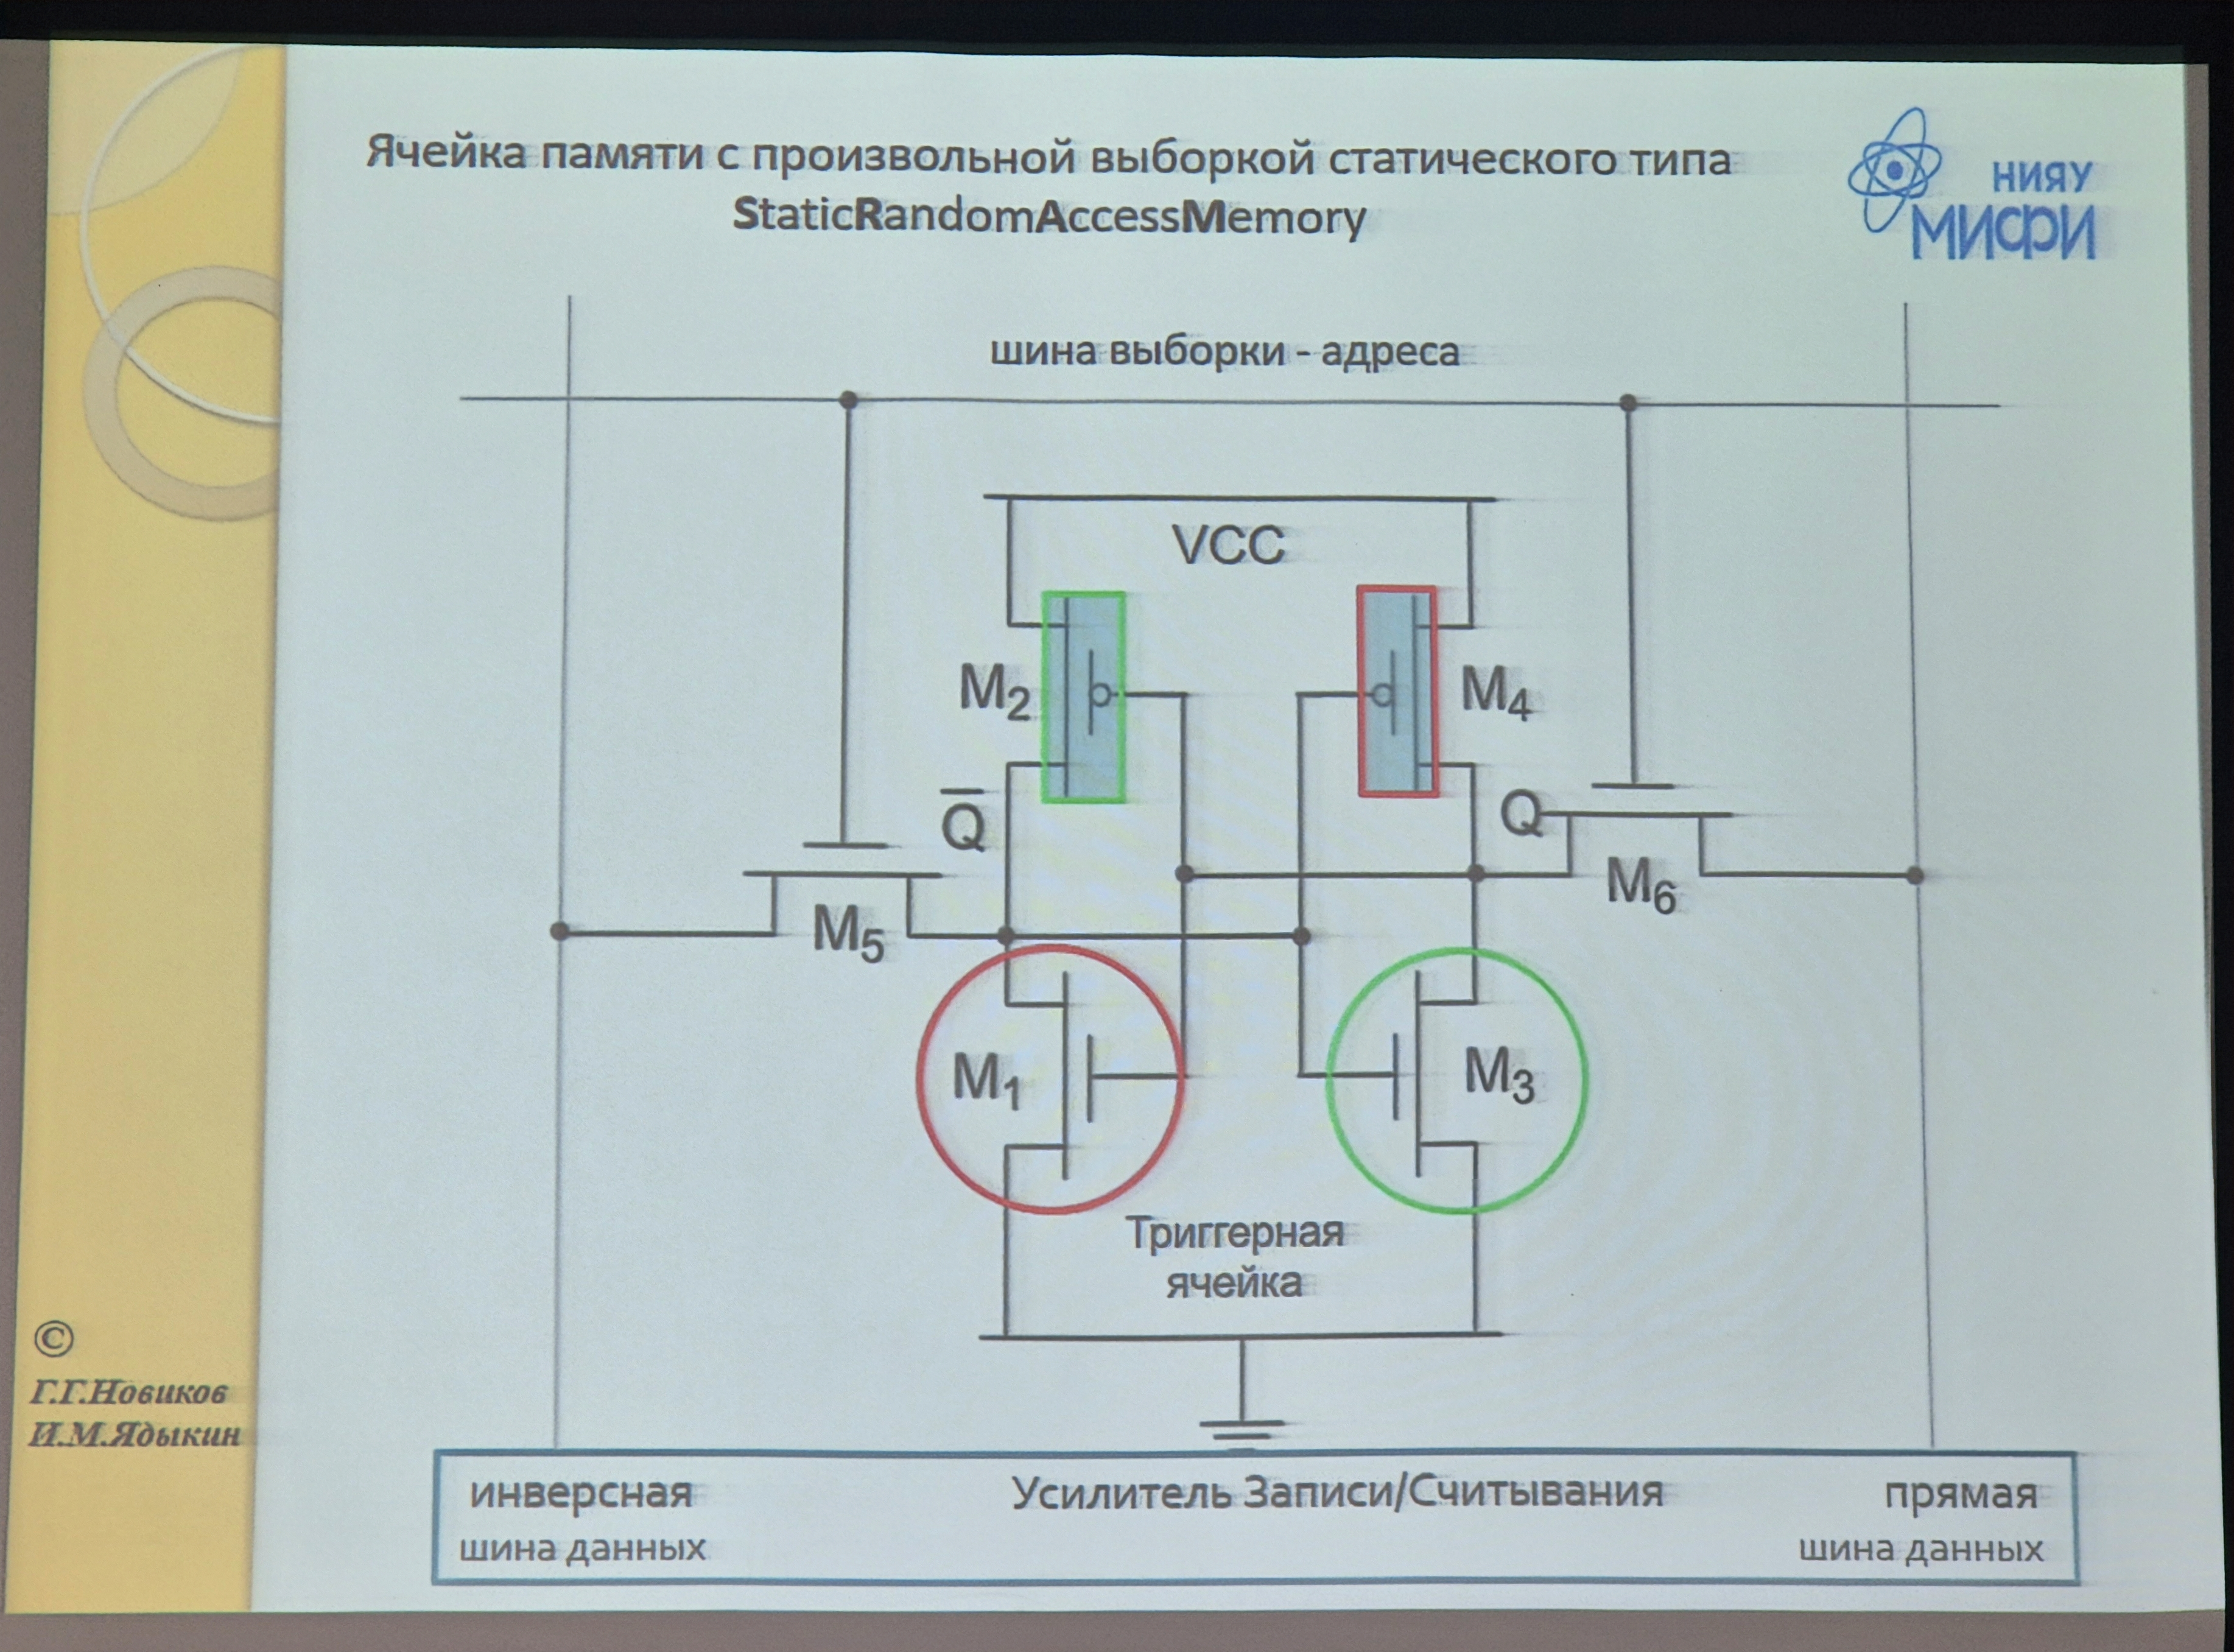
\includegraphics[width=0.7\linewidth]{images/SRAM.jpg}
\end{center}

Пара ... выход одного соединён со входом другого. 
Исключает возможность прямого тока от шины питания к земле. Реализован на полевых транзисторах. Хранит только до тех пор, пока есть питание. 
Функции выборки: M5, M6. Они подключены к плечам ячейки и будучи открыты шиной выборки соединяют выбранную ячейку с усилителем, подавая туда 2 сигнала противоположной полярности.\\

Зелёненькое и красненькое на слайдах меняется, поэтому биистабильно :)))\\

Здесь плохо, что ячейка хранит очень мало. 6 транзисторов на 1 бит.\\
Альтернитивный вариант динамическое запоминающее устройство на полевом транзисторе. 

\subsection{Одно-транзисторная ячейка памяти с произвольной выборкой динамического типа.}
\begin{center}
	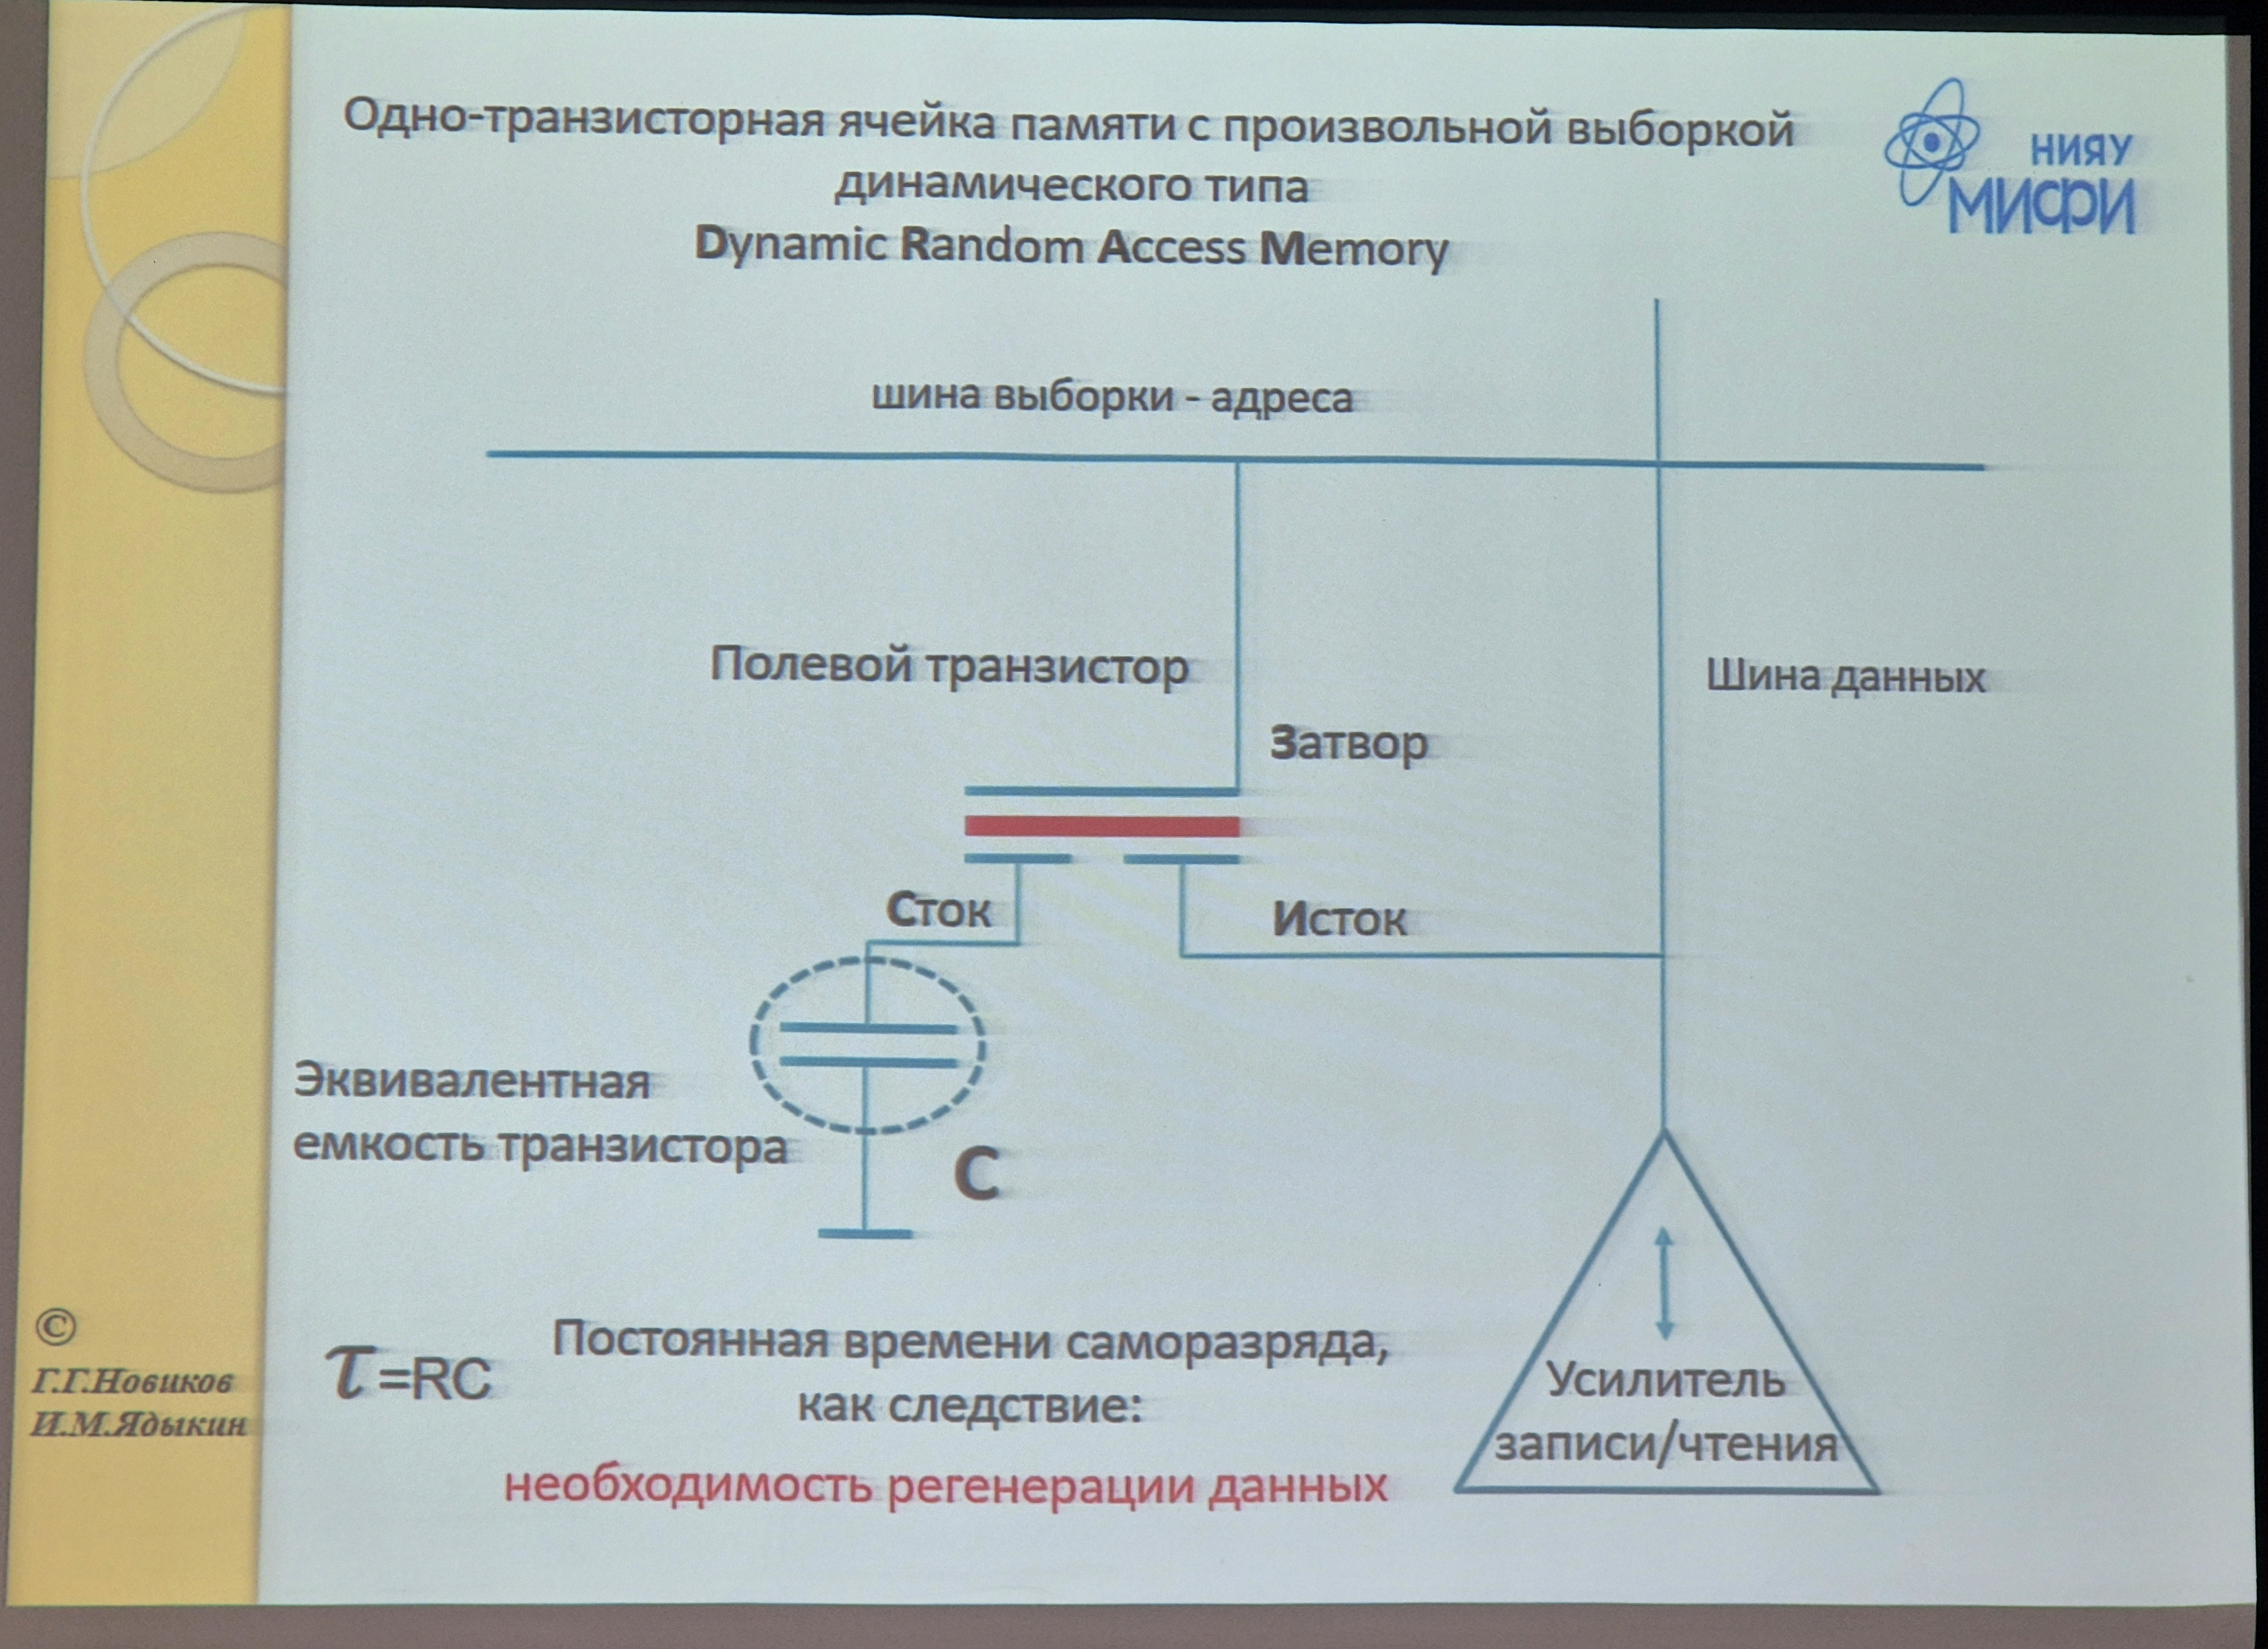
\includegraphics[width=0.7\linewidth]{images/DRAM.jpg}
\end{center}

Можно использовать конденсатор в качестве элемента хранения.
\begin{center}
	\includegraphics[width=0.7\linewidth]{images/Кондей и полевой транзистор.jpg}
\end{center}
Эквивалентная схемма с открытым транзистором и подключённый к усилителю, а затем закроем транзистор. Если опять открыть, то заряд потечёт в усилитель.\\
Но так как это полуизолятор мы можем повесить дополнительное сопротивление и со временем заряд стечёт и информация будет потеряна. Чтобы этого не произошло нужно считать её, записать и делть это постоянно. \\
Тоесть хранение информации в такой ячейке происходит динамически и требует постоянного чтения и записи (регинирации информаии). 
Почти 90\% всем ЗУ устроены так. \\
Разреженная регинерация - регинерация не всего массива, а только тех, кто нужен. Любое обращение к ячейке вызывает регинирацию.
\\ \\
\section{Лекция 10 от 06.11.2025.}
Вопросики:\\
Чем отличается память от склероза? В том, что на экзамене от всё забудет :(\\
Какие 4 операции есть в ЗУ? \\
В каком виду ЗУ в процессе хранения необходимо слово выборка? - Регинирация памяти. Динамическая память. \\
Что такое регенирация? - чтение и обратная запись того, что прочли.\\
А каком виде ЗУ так же требуется записывать после простения? - В ЗУ на основе фееритового сердечника из-за разрушающего свойства. \\
В какой метрике среда хранения полупроводникового ЗУ с произвольной выборкой? - двумерный массив. \\
Что такое хорошо, а что такое плохо, когда речь о ячейке статического типа? Весь тот гемор с обращением динамически к памяти не нужен. \\
Чем больше ёмкость тем дольше он будет хранить в цикле регинерации. \\


\subsection{АЛУ}
\begin{center}
	\includegraphics[width=0.5\linewidth]{images/АЛУ.jpg}
\end{center}

Выполняет арифмитические и логические операции. Для арифмитеческих операций необходимо (по Нейману) иметь сумматор, но могут быть и дополнительные ускорители процессов вычисления. \\
Минимальное число сумматоров, которые необходимы для работы ЭВМ - 1.\\

Для логических же операций необходимы:
\begin{itemize}
	\item Логические элементы (минимально нуже базис)
	\item Дополнительное оборудывание, которое могло бы выбрать какую из операций необходимо выполнить. 
\end{itemize}

Операции АЛ выполняются над \textbf{операндами} - число участвующее в А или Л опреации.\\
Схемма сумматора не обладают свойством сохранять свой состояние в отличие от ЗУ. \\
Комбинационная схема - схема значение которой есть только тогда, когда на вход поданы элементы. \\

Необходимо добаыить устройтсво для хранения операндом размером 1 (регистр). На схеме это ригистры операнда A и B. \\
Выходы регистров подключены к входам блока операций, а входы к тому месту где живут операнды (в памяти) соединяются магистралью с ЗУ. \\
Результаты хранятся в памяти (записывается из регистра результата). 

Дополнительная обратная связь между регистром результата и ... позволяет использовать результат в следующем вычислении. Появляется регистр аккумулятор (накапливающий). \\
Нужно указать АЛУ какую операцию выолнить. Это указание несёт в себе \textbf{коп} - код операции - число определяющее номер операции в списке возможных операций. 

Признаки результатов не нарисовали и мстное устройство управления ( в это не лезем ). \\

\subsection{Одноразрядный полный комбинационный сумматор}
	\includegraphics[width=0.5\linewidth]{images/Full adder.jpg}
% \includegraphics
Нужно сделать из него сумматор многоразрядный последовательный сумматор.
\subsection{Многоразрядный последовательный сумматор}
	\includegraphics[width=0.5\linewidth]{images/Многоразрядный сумматор.jpg}
% \includegraphics
ВОкруг обычного сумматора распологаются 3 регистра. \\
РР - регистр результаты. \\
Однако идея данного устройтсва в том, что это регистры обладающие функцией сдвига кода. \\
Картинка с нарушениями нужна только для демонстрации. \\
Сдвиги происхлдят одновременно во всех 3 регистрах из-за управляющего сигнала. \\
Тригер типа D передаёт в следующий такт то, что было на его входе в теущем (D - delay). \\
Все имеют вход с буквой С - вход для сингаринизации. Подаётся сгнал синхронизации на все элементы которые должны выполнить действия одновременно. \\
Хорошо: объём оборудования весьма скромный ( 1 комбинационный сумматор и несколько регистров с функцией сдвига + триггер). \\

Плохо: Время выполнения суммиорования прямо записит от количества операндов (8 тактов для байта). 


\subsection{4-х разрядный комбинационный сумматор.}
	\includegraphics[width=0.6\linewidth]{images/4-ч разрядный сумматор.jpg}\\
Это уже кусочек схемы. Входы слева, выходы справа. Логическое распростронение сигналов слева направо, сверху вниз.
Для каждой пары разрядов свой собственный отдельный одноразрядный комбинационный сумматор. Так что вычисление суммы происходит одновременно за 1 такт. \\

Плохо: с переносом проблема. 

\section{Устройство управления}
Что делает? - Пораждает сигналы управляющие. \\
Из чего пораждает? - Исходя из программы. \\
Программа - алгоритм решения задачи, записанный с помощью команж ЭВМ. \\
Алгоритм - последовательность действий необходимые для решения задачи.\\ 
Устройство Управления формирует управляющие сигналы исходя из того, какую команду оно выполняет. Суть - выполнение команды программы. \\
Команда программы - число. 

Что такое формат? - смысловое значение присвоенное отдельным разрядам в двоичной записи. В нашем случае команды. \\
\includegraphics[width=0.5\linewidth]{images/Command Format.jpg}
\includegraphics[width=0.5\linewidth]{images/Command Format2.jpg}

\begin{enumerate}
	\item  Операционная часть
	\item Адресная часть 
\end{enumerate}

Всякая команда состоящая из этих частей имеет некоторый набор характеристик. 
Операционная часть команжы содержит в себе:
\begin{itemize}
	\item КОП (Код ОПерации - двоичное число идентифицирующее команду в системе команд ЭВМ) 
\end{itemize}

Какая связь между кодом операции и количество разрядов кода опреации: $2^n$ - Мощность .
Адресная часть:
\begin{enumerate}
	\item Адреса операндов, участвующих в этой команде. 
\end{enumerate}

\textbf{Адресация} - способ указания местаположения этого операнда в адресном поле команды.Способов этих можно придумать бесконечно. \\
\textbf{Основные способы адресации:}
\begin{enumerate}
	\item Когда адреса нет вообще. Неявная адресация. Нет указания куда помещать результат.\\
	\includegraphics[width=0.5\linewidth]{images/Adressing1.jpg}

	\item Непосредственная адресация. В адресном поле распологается сам операнд. \\
	\includegraphics[width=0.5\linewidth]{images/Adressing2.jpg}\\
	Чем команда меньше, тем быстрее она будет извлекаться. 
	\item Прямая адресация. 
	\item Регистровая адресация
	\includegraphics[width=0.5\linewidth]{images/Adressing3.jpg}\\
	\item Косвенная адресация\\
	\includegraphics[width=0.5\linewidth]{images/Adressing4.jpg}\\
		Адрес адреса операнда. Может быть построена на нескольких уровнях вложенности. 

\end{enumerate}


\section{Лекция 11. От 13.11.2025}
\subsection{Вопросики}
Что такое формат команд? - 2 части: операционная и адресная. В операционной - код операции (двоичное число, которое однозначно идентифицирует команду в системе команд)\\
С какой характеристикой ЭВМ связаня величина поля ввода операции? - Мощности системы команд эвм, что равно количеству команд в штуках.\\
Какая характеристика позволяет оценить количество полей в адресной части команды? - количество адресов (адресность)\\
Как называется то, что определяет способ записи местонахождения операнда в этом адресном поле - адресация или способ адресации. \\
Где следует искать операнд если использована непосредственная адресация - непосредственно в этом адресном поле. \\
А если адресация прямая - искать в оперативной памяти по адресной ячейки, который написан в адресном поле команды. \\
А если косвенное - искать адрес операнда в ячейке адрес которой указан в адресном поле команды. Адрес адреса операнда. \\
Поругайте мне косвеную адресацию - многократное обращание в памяти ( время докапывания до операнда (минимум 2 раза)). \\
О какой характеристики ЭВМ можно судить о величине адресного поля при использовании косвеной адресации - по объёму оперативной памяти.\\
Как сохранить косвеность и справиться с проблемами косвеной адресации? - использование варианта косвенойадресации, в котором хранится информация не в ячейке ОП, а в регистре, получается косвеная регистровая адресация. \\

\subsection{Регистровая адресация}
\begin{center}
	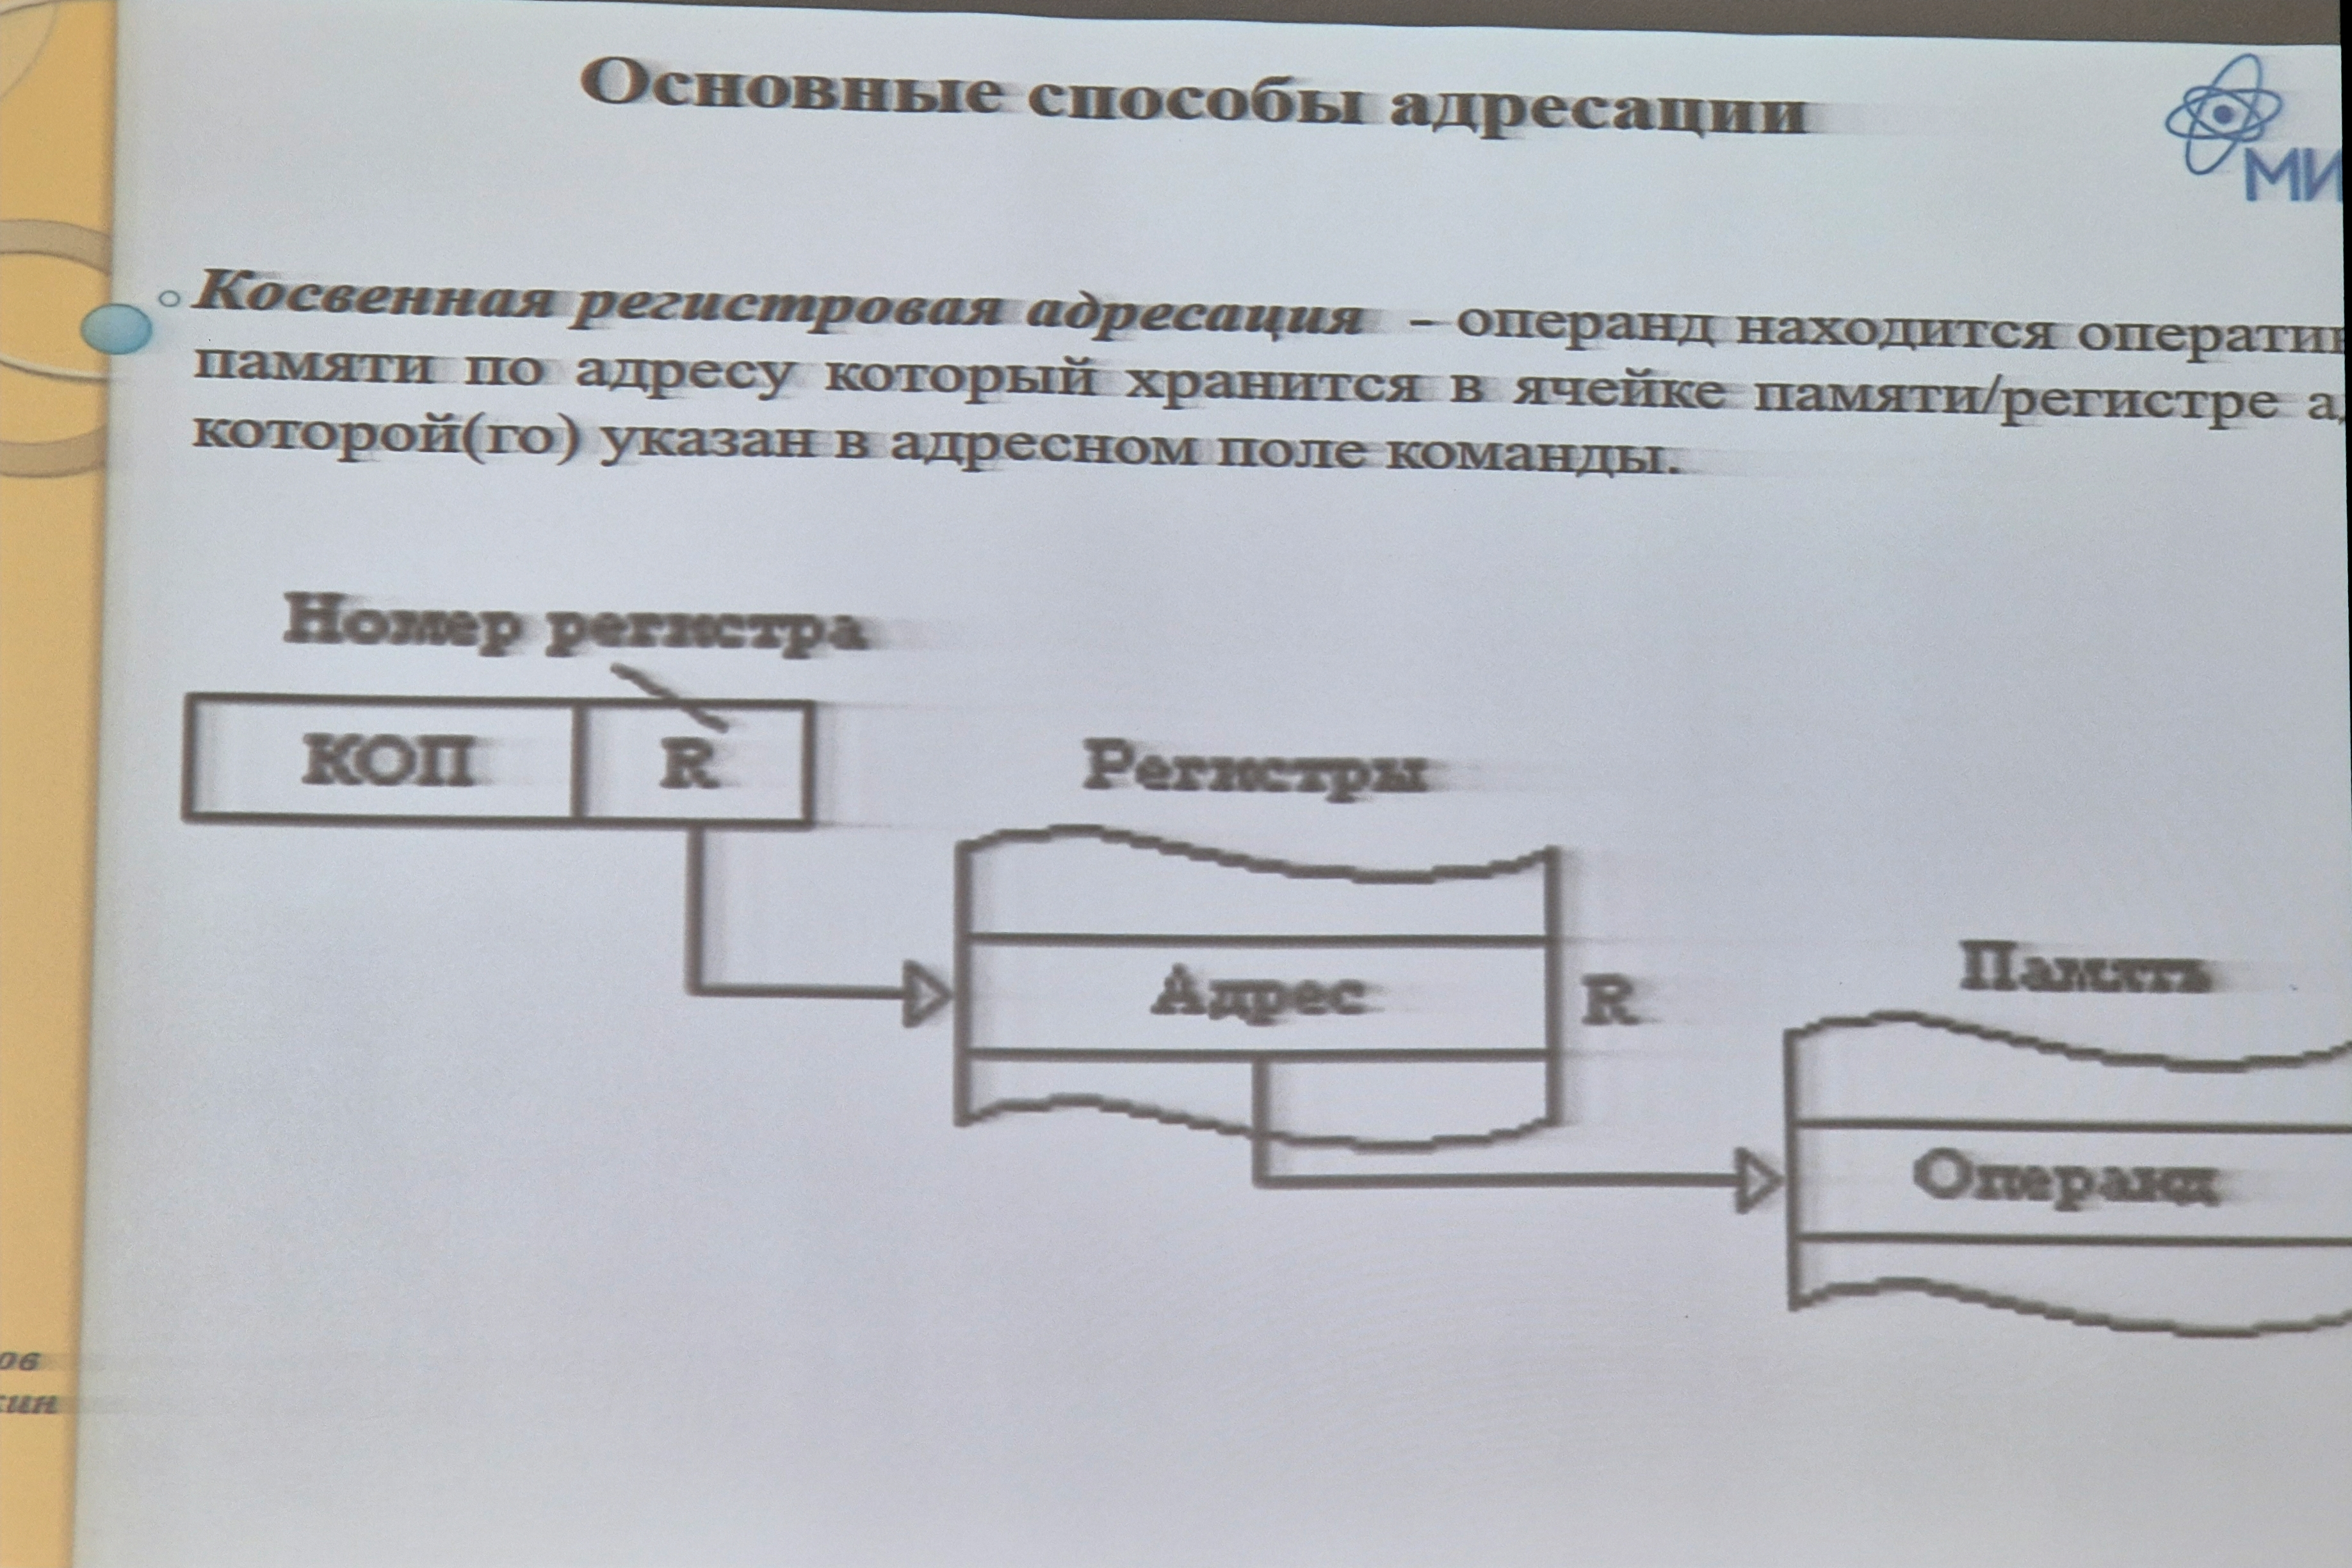
\includegraphics[width=0.5\linewidth]{images/Adressing5.jpg}
\end{center}
Скороть наивысшая. \\
1 обращение в регистровую память, 2 обращение по адресу, извлечённому из регистро обращаемся в ООП. Получаем все плюшки косвеной адресации. 

\subsection{относительная адресация}
\begin{center}
	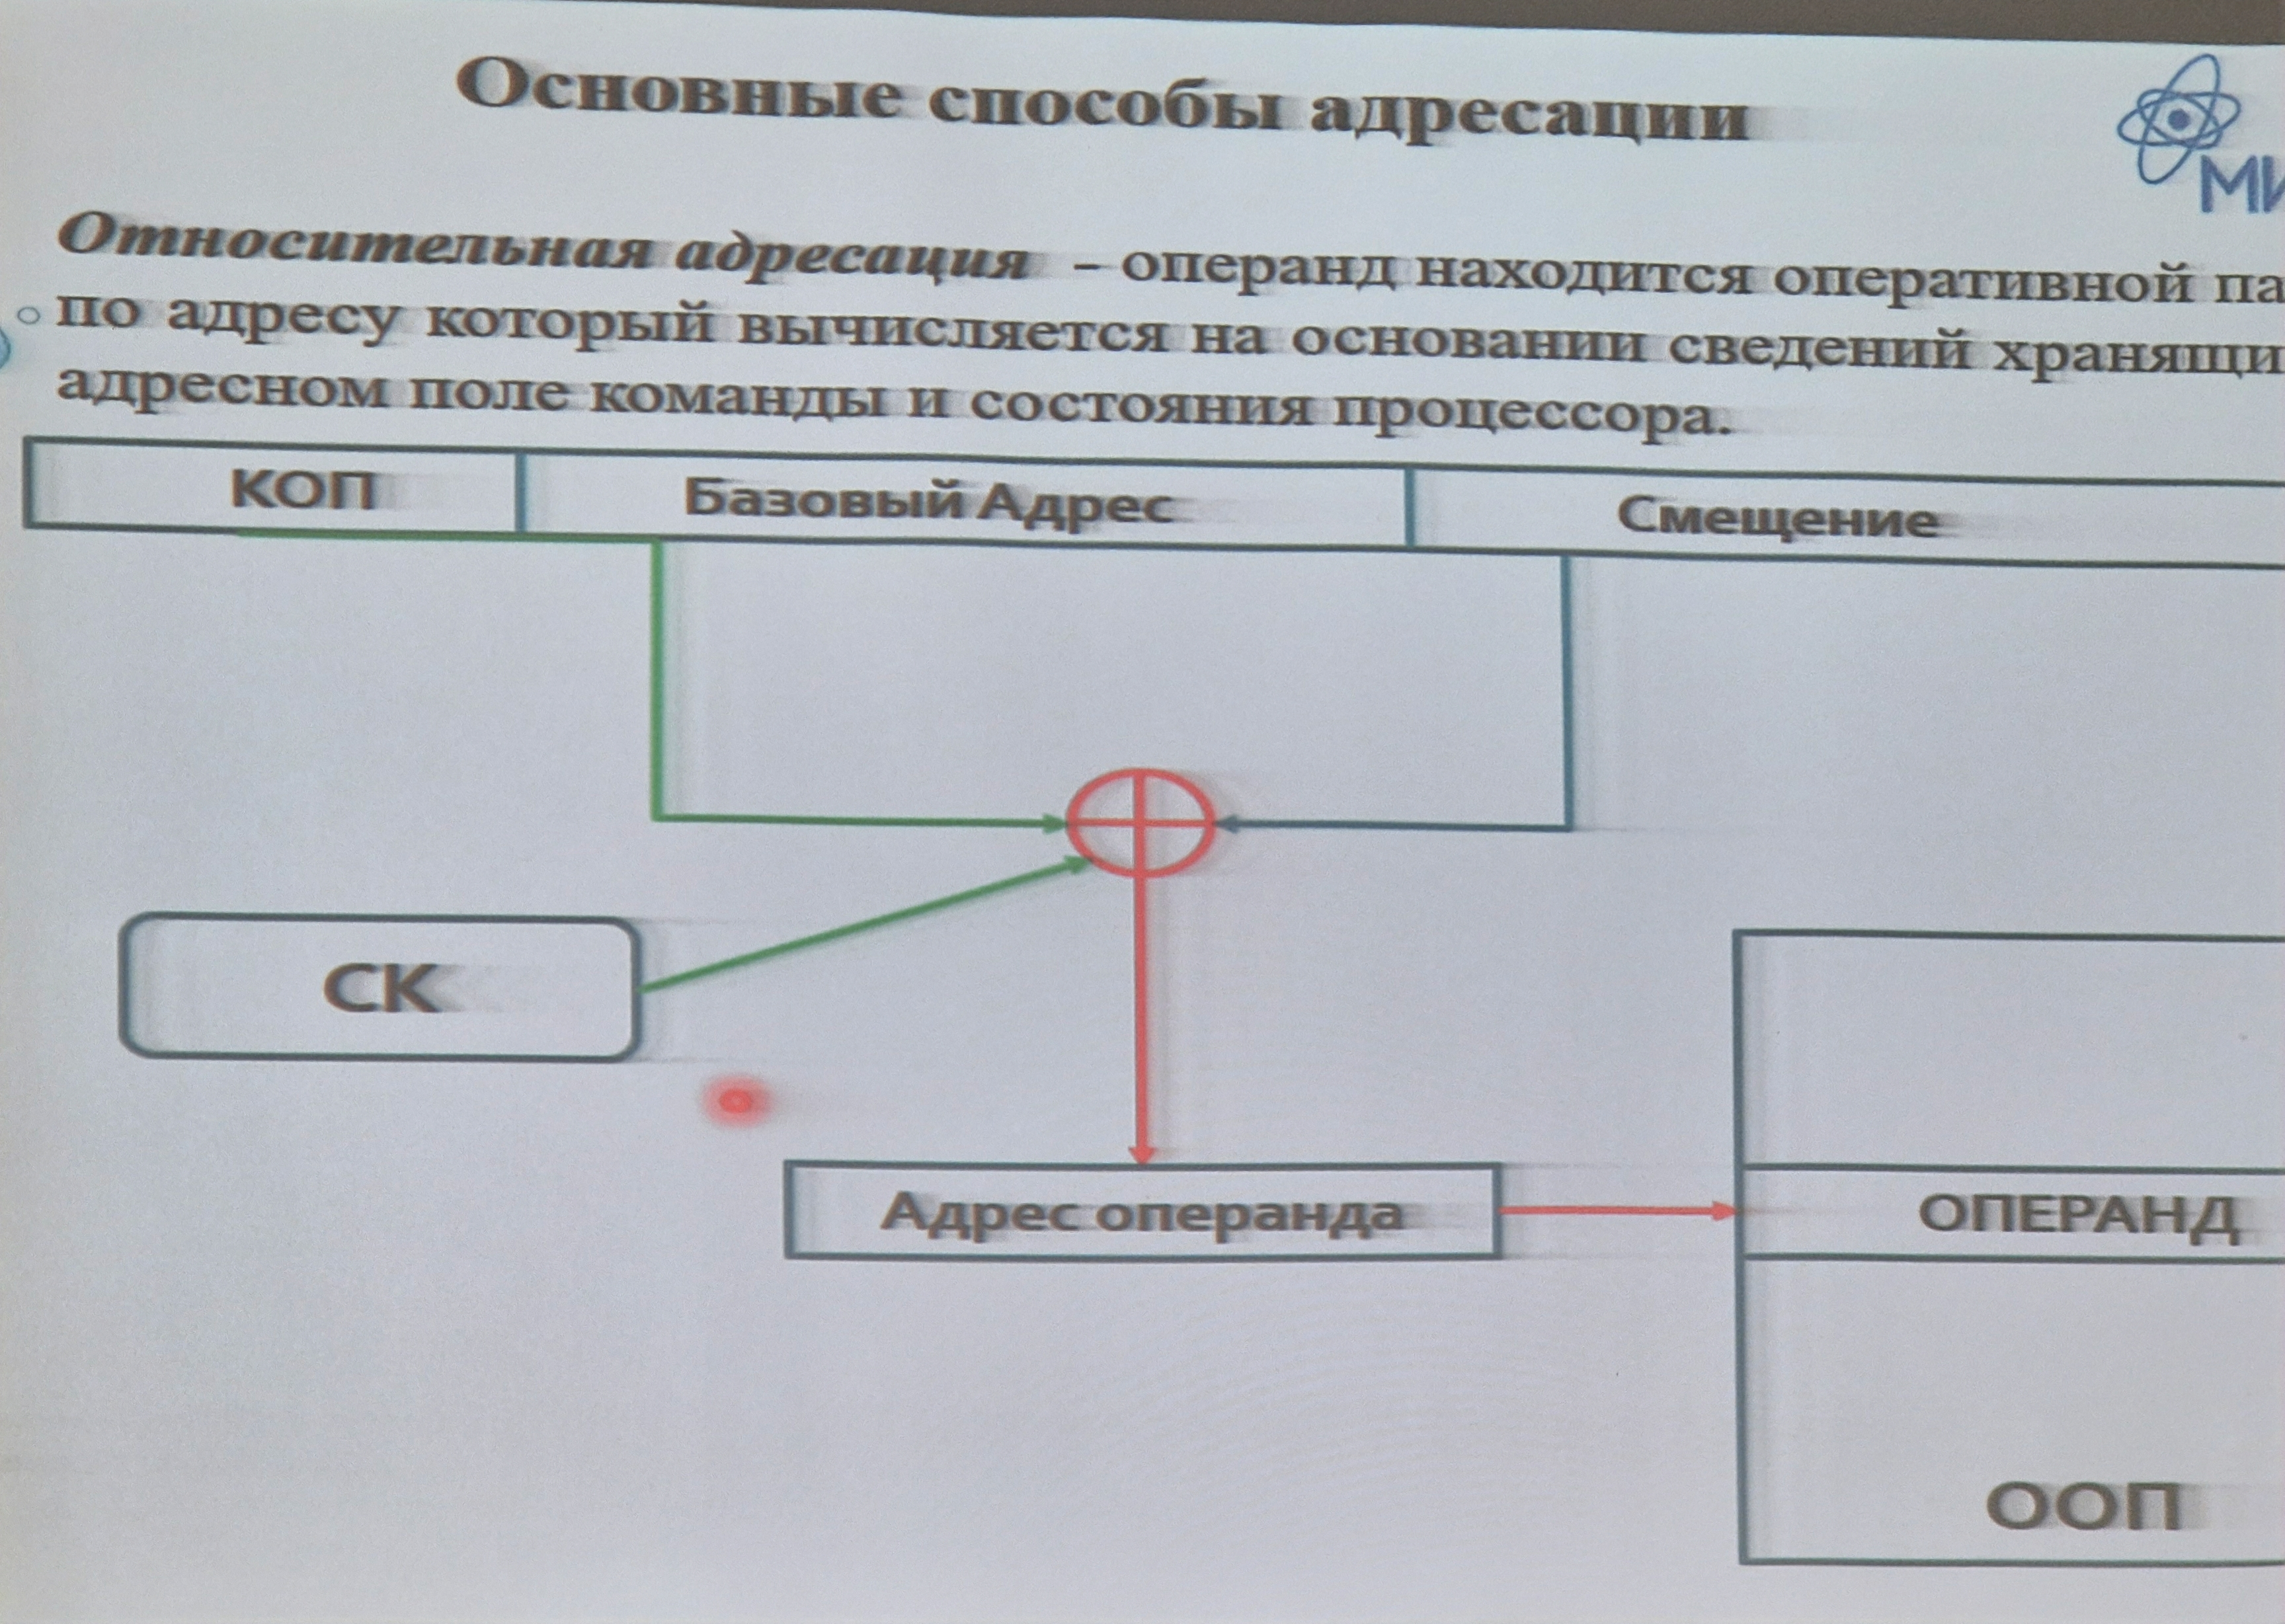
\includegraphics[width=0.5\linewidth]{images/Adressing6.jpg}
\end{center}
Местоположение операндов в памяти задаётся с помощью смещения относительно чего-то. Обычно относительно некоторого базового адреса. Т.о. получается, что при формировании адреса операнда используется суммирование, а именно сумма адреса базового и смещение. \\
Крестик на фото и есть суммирование. 

СК - счётчик команд - хранит следующую команду. Местонахождение операнда определяется относительно местонахождением команды. 
В момент, когда надо загрусить команду в память задаётся начальное смещение в виде точки, куда будет загружаться программа - классика при мультипрограмном режиме. 

\subsection{Автоинкриментная адресация}
\begin{center}
	\includegraphics[width=0.5\linewidth]{images/Adressing7.jpg}
\end{center}
Не что иное как косвенная/косвенная регистровая адресация, у которой адрес операнда может меняться путём увеличения инкримента на константу при каждом использовании этой команды.\\
Т.о. при запуске такой каманды в цикле получим последовательное обращение подряд идущих элементов (нужно например для массивов). \\
Существует в варианте инкримента и декримента - одно увеличивает, другое уменьшает. 

\subsection{Заключение по видам адресаций}
Адресаций может быть бесконечно много. Нужно знать неявную, прямую, косвеную, регистроваю, косвеную регистроваю, автоинкримент декримент, относительную адресации. 


% Команда должна привести к набору управляющих сигналов. 

\subsection{Трёхадресная ЭВМ}
\begin{center}
	\includegraphics[width=1.0\linewidth]{images/3AdressEVM/3adress.jpg}
\end{center}
Состоит из:
\begin{enumerate}
	\item Арифметико-Логическое Устройство. В нём логические элементы. На вход принимает операнды и пораждается результат (РР) и признок результата (РПр). 
	\item Оперативное Запоминающее Устройство. Функции: хранение, чтене, запись, выборка. 
	\item Устройство Управления. \\
	Оно разделяется на 2 основные часи:
	\begin{enumerate}
		\item РК - Регистр команды. Обращаем внимание на то, что речь про 1 и тоьлко 1 команду. \\
		Число, которое хранится в этом регистре представляет собой команду. Формат этого числа - формат команды. \\
		Структура регистра команды определяется опаратной реализацией формата команды. Число записанное туда как раз и занимает поля формата команды и содержит всё что там полагается. Могут обитать 3 адреса: a, b, c, а также сам Код ОПерации. \\
		Команд много, а регистр может хранить 1 единственную программу - выполняемую в данный момент времени. Именно по этой причине \textbf{Функция регистра команды}: хранение команды в процессе её выполнения (той самоё 1 единственной). \\
		Логичные вопросы, которые возникают:
		\begin{itemize}
			\item Как команда попадает в регист команды?
			\item Как команды в памяти превращаются в программу?
		\end{itemize}
		\textbf{Программа} - алгоритм для решения задачи, записанный командами ЭВМ. \\
		
		\textbf{Способ адресации команд программы} (не путать со способами адресации операндов) по сути способ связовании команд в программу: 
		\begin{enumerate}
			\item \textbf{Принудительная адресация программ команд программы.} \\
				Суть заключается в том, что команда в своей адресной части имеет адресное поле с адресом следующей команды (обычно где-то в конце). Получается, что текущая команда выполняемая в данный момент несёт в себе адрес следующей программы. Получается структура, которая называется \textbf{связанный список} (блок-чайн без шифрования ;) ).\\ 
				Плюсы и минусы такого способа:
				\begin{itemize}
					\item Никаких усилий для вычисления адреса следующей программы не нужно. команды могут распологаться как угодно в любых ячейках памяти. 
					\item Занимает место. Приходится тащить поле размером с адрес основной оперативной памяти, а команд много, так что количество необходимой памяти сильно увеличивается. 
				\end{itemize}
		\item \textbf{Естественная адресация команд программы.} \\
			Берётся память (одномерный массив ячеек или же вектор) и в неё последовательно в том порядке, в котором они должны выполняться вносятся команды. При таком способе к конструкции добавляется устройство, хранящее адрес команды и обладающее возможностью инкремента для добавления некоторой $\Delta$, что является размером данной команды, - это называется \textbf{счётчик команд}. \\
			Плюсы и минусы такого способа:
			\begin{itemize}
				\item Избавляемя от поля для команды, значит не приходится тратить лишнюю память.
			\item Нужно класть команды в ячейки строго в порядке выполнения и необходимо потратить дополнительное оборудование для формирования адреса следующей команды + небольшое время добавления дельты к адресу. 
			\end{itemize}
		\end{enumerate}
		Преимущество в размере команды преволирует над первым способом, поэтому обычно используется естестенная адресация. \\
		В трёхадресной ЭВМ используется именно естественная адресация (видно счётчик команд ;) )\\

		\textbf{Счётчик команд} - Instruction Pointer - IP - указатель на команду.
		\begin{center}
			ОЧЕНЬ ВАЖНО! Никакой связи IP с интернет протоколами на зачёте нет.
		\end{center}
		
		Счётчик команд передат адрес следующей команды на Регистр Адреса ЗУ, указывая на ячеёку памяти, где она хранится и считанное по этому адресу число загружается в Регистр Команды. 
		\item Управление сигналами: \\
			Помним, что Устройство Управления решает 2 задачи: что делать и когда это делать.\\
			Что делать понятно из команды, расположенной в регистре команд, код операции которой передаётся в дешифратор кода операции. Смысл этого действия в том, чтобы сообщить той части, которая формирует сигналы (Блоку Управления ОПерациями), какая это команда. \\
			
			Вопросом коaгда занимается Датчик Сигнала (служба времени было-бы красивее @Новиков). 
\begin{center}
	\includegraphics[width=0.5\linewidth]{images/3AdressEVM/Time}
\end{center}
			Что такое время с точкизрения физики? \\
			Время - это физическая величина, которую не определить, но оно обладает свойствами: время течёт равномерно и непрерывно. \\
			Заменяем физическое время на \textbf{время дискретное}.\\
			Для этого мы испльзуем генероватор квантов (сигналов) и предствляем время при помощи импульсов. \\
			\textbf{Импульс} - изменение во времени состояние электрического сигнала несущего значение логической переменной из исходного состояние в противоположное. \\
			Пучть 1 импульс будет равен 1 \textbf{кванту времени} или же по другому 1 \textbf{такту}, тогда другой импульс будет другим тактом и т.д.\\

			А между импульсами ничего нет. Тогда в нашем новом дискретном времени все события происходят в этих тактах. Поэтому эти такты мы можем пронумеровать (t - сейчас, t+1 - следующий момент времени, t + 2, ...). Можно и в обратную сторону (t - 1, t - 2, ...). \\
			
			Порадив такое квантовое время и поняв, что события происходят только в тактовый импульс мы становимся хозяевами того, что происходит в каждый конкретный импульс. Но физическое время никуда не делось и в нём происходят импульсы, а раз они формируются в физическом времени, то у них есть тот же небор характеристик, что и у импульсного сигнала: 
			\begin{itemize}
				\item Длительность
				\item Амплитуда
				\item Фронт
				\item Период ($T$)- время между одинаковыми частями 2 соседних импульсов. 
				\item Частота (тактовая частота) - величина обратная периоду: $F = \frac{1}{T}$. Её порождает генератор тактовых импульсов.\\
			Изменяя частоту мы изменяем насколько часто будут происходить события в нашем устройстве. Чем быстрее тактовая частота тем быстрее работает устройство.\\
			\end{itemize}

	Мы должны иметь возможность внутри циклы выполнения команды указывать на моменты времени, в которые должны выполняться те самые действия, которые будут повторяться. Т.о. мы должны не только разбить время на кванты, но и имет возможность выбирать (наверное тут было: какой квант выполнять). В этом помогает \textbf{распределитель импульсов цикла}.  

\begin{center}
	\includegraphics[width=0.5\linewidth]{images/3AdressEVM/TimeDiagram}
\end{center}
	
	В этом примере мы получили, что у нас есть 4 сигнала, которые связаны с друг с другом так, что импульсы на тактах 1, 2, 3, 4 будут соответствовать ...\\
	Подавая с линии A выполнится 1 такт, а на линии C - 3 такт. \\

	Схематехнически это выглядит так:
	\begin{center}
		\includegraphics[width=0.7\linewidth]{images/3AdressEVM/TimeDiagram2}
	\end{center}
	\end{enumerate}
	Вот тут у меня плохо получилось:\\
	Каждый тактовыё импульс изменяет состояние счётчика на +1. 
	Дешифратор преобразует позиционный код в унитарный. \\
	Пришёл импульс, счётчик переключился, одразовался один ноль (единица двоичная) единичка на дешифраторе переместилась на 1 выход. След на дешифратор, счётчик на 2. 1 не выходе дешифратора переместилась на выход номер 2. Т.о. прошёл всё да в пизду. \\

	Дешифратор кода определяет какие именно импульсы нужны для реализации команды. Объединяет всё блок управления операциями (что и когда). Из него во все стороны и формируются i-е управляющие сигналы, подключающиеся к устройствам. 
\end{enumerate}






\end{document}

